\section{Results}

\subsection{Word Occurences}

In the first table \ref{table:table_motility} The results reveal a strong asymmetry between the two conceptual fields. Terms related to motility are almost absent from both corpora, while accessibility vocabulary is frequent and well represented. This suggests that Swiss spatial planning discourse focuses primarily on infrastructural and material dimensions of mobility. The human, cognitive, and motivational aspects that define motility are not expressed in the language of planning documents. Mobility appears as something provided through networks and infrastructure rather than as a capability that individuals develop and use. The conclusion is the same for French and German.

The same pattern is visible in the analysis of time-related terms in table \ref{table:table_time}. References to physical or objective time largely outweigh those to perceived or subjective time. Travel time is described as a variable to be reduced, optimized, or measured. Few terms evoke comfort or satisfaction. This indicates that time is approached mainly as an operational parameter rather than a human experience. But the contrast is not as dramatic as for motility between the two perspective.

Taken together, these findings show that planning discourse remains centered on measurable, supply-side factors. The subjective dimensions of mobility, including skills, motivation, and perception, are weakly represented not to say absent. The language used in official documents thus reflects and reinforces a narrow view of mobility, oriented toward infrastructure and performance rather than individual capacities and experiences.
\begin{table}[H]
\centering
\caption{Frequency of mobility-related terms in French and German corpora (aligned by conceptual field: Motility vs Accessibility)}
\resizebox{\textwidth}{!}{
\begin{tabular}{@{}llS[table-format=5.0]lS[table-format=5.0]S[table-format=5.0]@{}}
\toprule
\textbf{Category} & \textbf{FR term} & \textbf{FR hits} & \textbf{DE term} & \textbf{DE hits} & \textbf{Total} \\
\midrule
\multicolumn{7}{l}{\textbf{Motility}} \\
\midrule
 & aptitude mobilité & 3 & Bewegungsfähigkeit & 3 & 6 \\
 & capital mobilité & 0 & Mobilitätskapital & 0 & 0  \\
 & habitus mobilité & 0 & Mobilitätshabitus & 0 & 0 \\
 & autonomie déplacement & 0 & Bewegungsautonomie & 0 & 0  \\
 & apprentissage mobilité & 0 & Mobilitätslernen & 0 & 0  \\
 & stratégie déplacement & 1 & Mobilitätsstrategie & 14 & 15  \\
 & compétence & 159 & Orientierungskompetenz & 0 & 159  \\
 & représentation espace & 0 & Raumvorstellung & 0 & 0 \\
 & motivation mobilité & 0 & Mobilitätsmotivation & 0 & 0  \\
 & (valeur) symbolique mobilité & 0 & Symbolisch Mobilität & 0 & 0  \\
\midrule
\textbf{Subtotal (Motility)} &  & 163 &  & 17 & 180 \\
\midrule
\multicolumn{7}{l}{\textbf{Accessibility}} \\
\midrule
 & accessibilité & 284 & Erreichbarkeit & 207 & 491  \\
 & qualité desserte & 159 & Versorgungsqualität & 3 & 162  \\
 & intégration transport & 3 & Verkehrsintegration & 0 & 3  \\
 & coût & 304 & Kosten & 321 & 625 \\
 & disponibilité transport & 1 & Verfügbarkeit verkehrsmittel & 1 & 2 \\
 & infrastructure & 1109 & Infrastruktur & 738 & 1847  \\
 & centralité spatial & 0 & räumlich zentralität & 0 & 0  \\
 & inégalité accès & 0 & erreichbarkeitsgerechtigkeit & 0 & 0  \\
 & budget mobilité & 0 & mobilitätsbudget & 0 & 0 \\
 & réseau transport & 331 & verkehrsnetz & 100 & 431  \\
\midrule
\textbf{Subtotal (Accessibility)} &  & 2187 &  & 1370 & 3557  \\
\bottomrule
\end{tabular}
}
\label{table:table_motility}
\end{table}


\begin{table}[H]
\centering
\caption{Frequency of time-related terms in French and German corpora (aligned by concept)}
\resizebox{\textwidth}{!}{
\begin{tabular}{@{}llS[table-format=5.0]lS[table-format=5.0]S[table-format=5.0]@{}}
\toprule
\textbf{Category} & \textbf{FR term} & \textbf{FR hits} & \textbf{DE term} & \textbf{DE hits} & \textbf{Total}  \\
\midrule
\multicolumn{7}{l}{\textbf{Physical / Objective Time}} \\
\midrule
 & Minute & 132 & Minute & 207 & 339 \\
 & Heure & 192 & Stunden & 0 & 192 \\
 & Durée & 48 & Dauer & 2 & 50  \\
 & Vitesse & 158 & Geschwindigkeit & 17 & 175  \\
 & Rapidité & 17 & Schnelligkeit & 0 & 17  \\
 & Ponctualité & 7 & Pünktlichkeit & 7 & 14  \\
 & Retard & 4 & Verspätung & 1 & 5  \\
 & Kilomètre & 180 & Kilometer & 28 & 208  \\
 & Ralentissement & 3 & Verlangsamung & 3 & 6  \\
 & Cadence & 160 & Taktfrequenz & 0 & 160  \\
\midrule
\textbf{Subtotal (Physical)} &  & 901 &  & 265 & 1166 \\
\midrule
\multicolumn{7}{l}{\textbf{Perceived / Subjective Time}} \\
\midrule
 & Attente & 28 & Wartezeit & 3 & 31  \\
 & Stress & 0 & Fahrstress & 0 & 0  \\
 & Confort & 15 & Komfort & 0 & 15  \\
 & Expérience & 20 & Erfahrung & 20 & 40  \\
 & Ressentir / Percevoir & 5 & Wahrnehmung & 5 & 10 \\
 & agréable & 10 & angenehm & 2 & 12  \\
 & Satisfaction usager & 0 & Fahrgastzufriedenheit & 0 & 0  \\
 & Temps Réappropriable & 0 & Zeitnutzung & 0 & 0  \\
 & temps valorisé & 0 & bewertete Zeit & 0 & 0  \\
 & Temps vécu & 0 & gelebte Zeit & 0 & 0  \\
 & Bien-être (mobilité) & 0 & Wohlfühlmobilität & 0 & 0  \\
\midrule
\textbf{Subtotal (Subjective)} &  & 78 &  & 30 & 108  \\
\bottomrule
\end{tabular}
}
\label{table:table_time}
\end{table}


\subsection{Analysis of PCA Results related to time}

As shown in Figure~\ref{fig:PCA_FR_time}, the French corpus reveals a marked separation 
between objective and subjective temporal notions. Terms associated with measurable, 
operational time such as \emph{vitesse}, \emph{minute} and \emph{kilomètre} are strongly 
loaded on the first principal component, highlighting their dominant role in structuring 
the discourse. In contrast, experiential notions like "stress", "confort", 
"attente" or "ressenti" cluster closely together and are much less present as seen in table \ref{table:table_time}. The cantonal points occupy a dense region in the lower-left quadrant, suggesting a relatively homogeneous and technically oriented use of time-related vocabulary across French-speaking institutional texts, with the exception of Bern, which leans more toward "cadence", "durée" and "vitesse" instead of "heure", "minute" or "kilomètre". The author theorizes that this may be due to a translation from German for the Bern plan, which is the only one available in both languages.

Figure~\ref{fig:PCA_DE_time} shows that the German corpus follows the same pattern, but 
with an even stronger emphasis on objective temporal measures. Terms such as 
"Geschwindigkeit" and "Kilometer" form the major axis of variation and clearly structure the first component. Subjective notions like "Erfahrung" or "angenehm" rarely appear and cluster together, suggesting that they contribute weakly to the overall variance. The clustering of cantonal abbreviations in a compressed zone indicates limited lexical differentiation among German-speaking institutional texts, reinforcing 
the observation that technical and operational understandings of time dominate the 
discourse, while experiential dimensions remain secondary with the main fracture being the usage of time versus distance.

\begin{figure}[H]
    \centering
    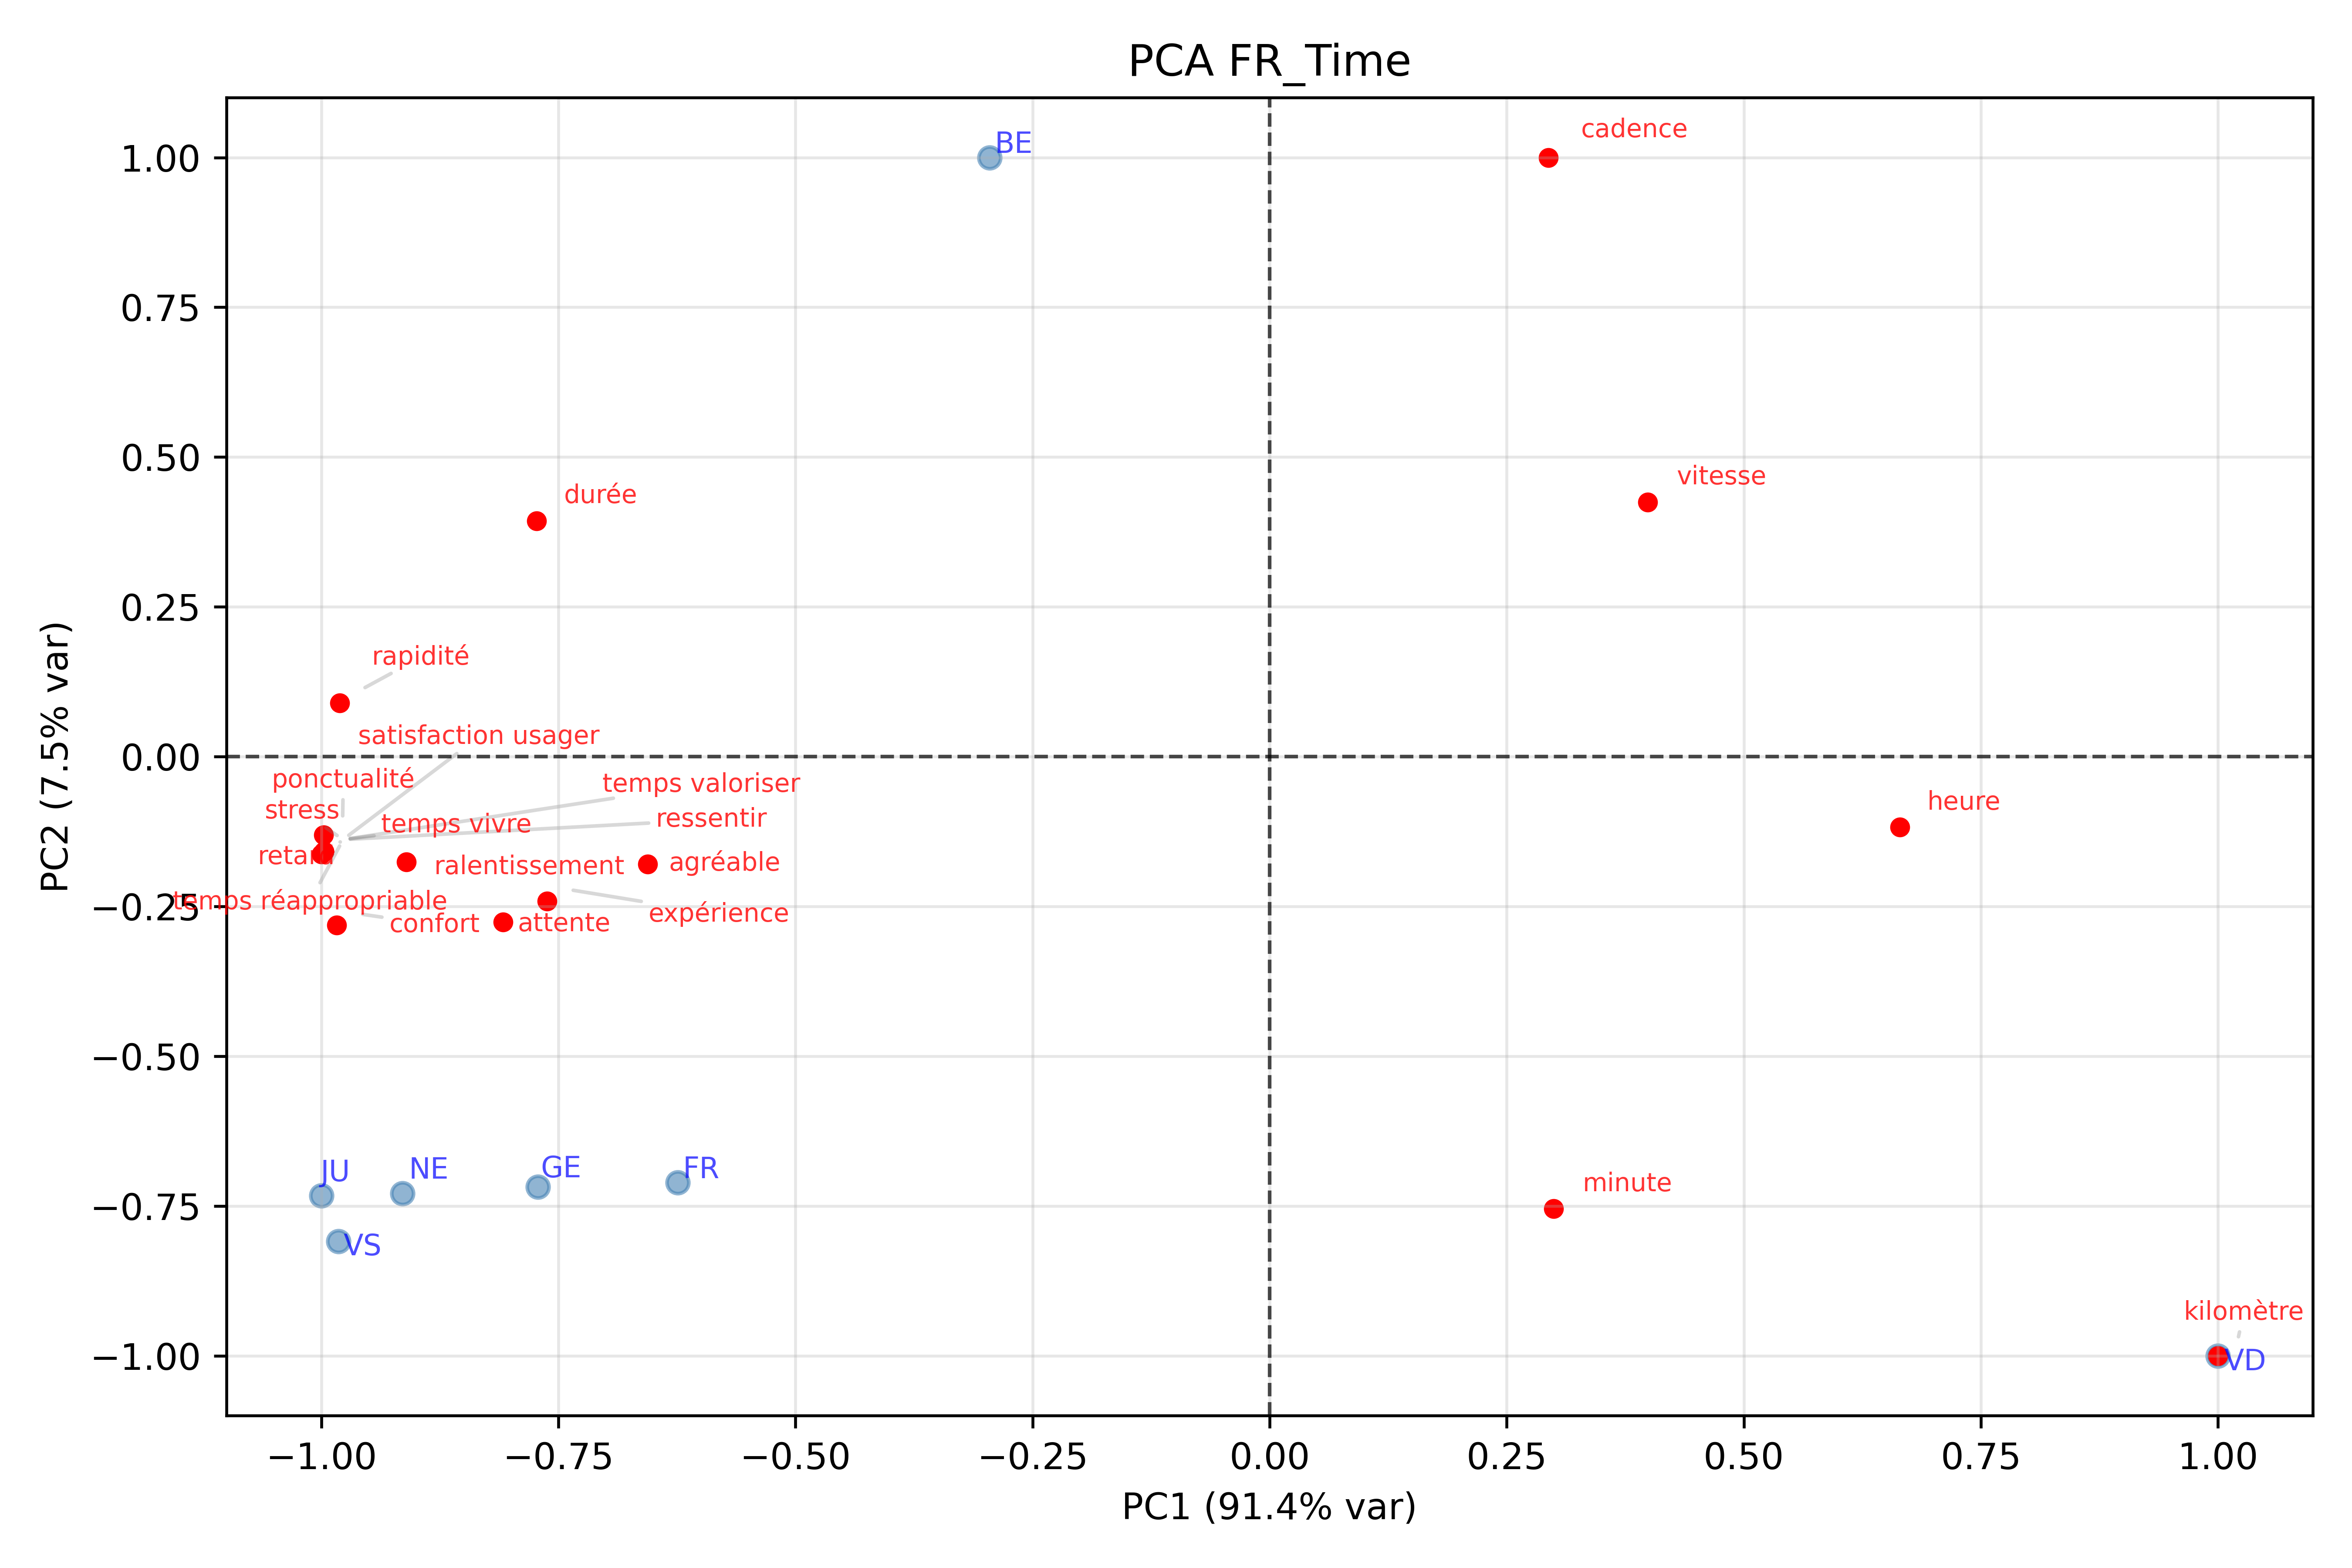
\includegraphics[width=0.95\linewidth]{Analysis/software/result/PCA_FR_Time.png}
    \caption{\textit{The French PCA highlights the dominance of quantifiable temporal notions, while 
subjective or experiential terms remain marginal in their contribution to variance.}}
    \label{fig:PCA_FR_time}
\end{figure}

\begin{figure}[H]
    \centering
    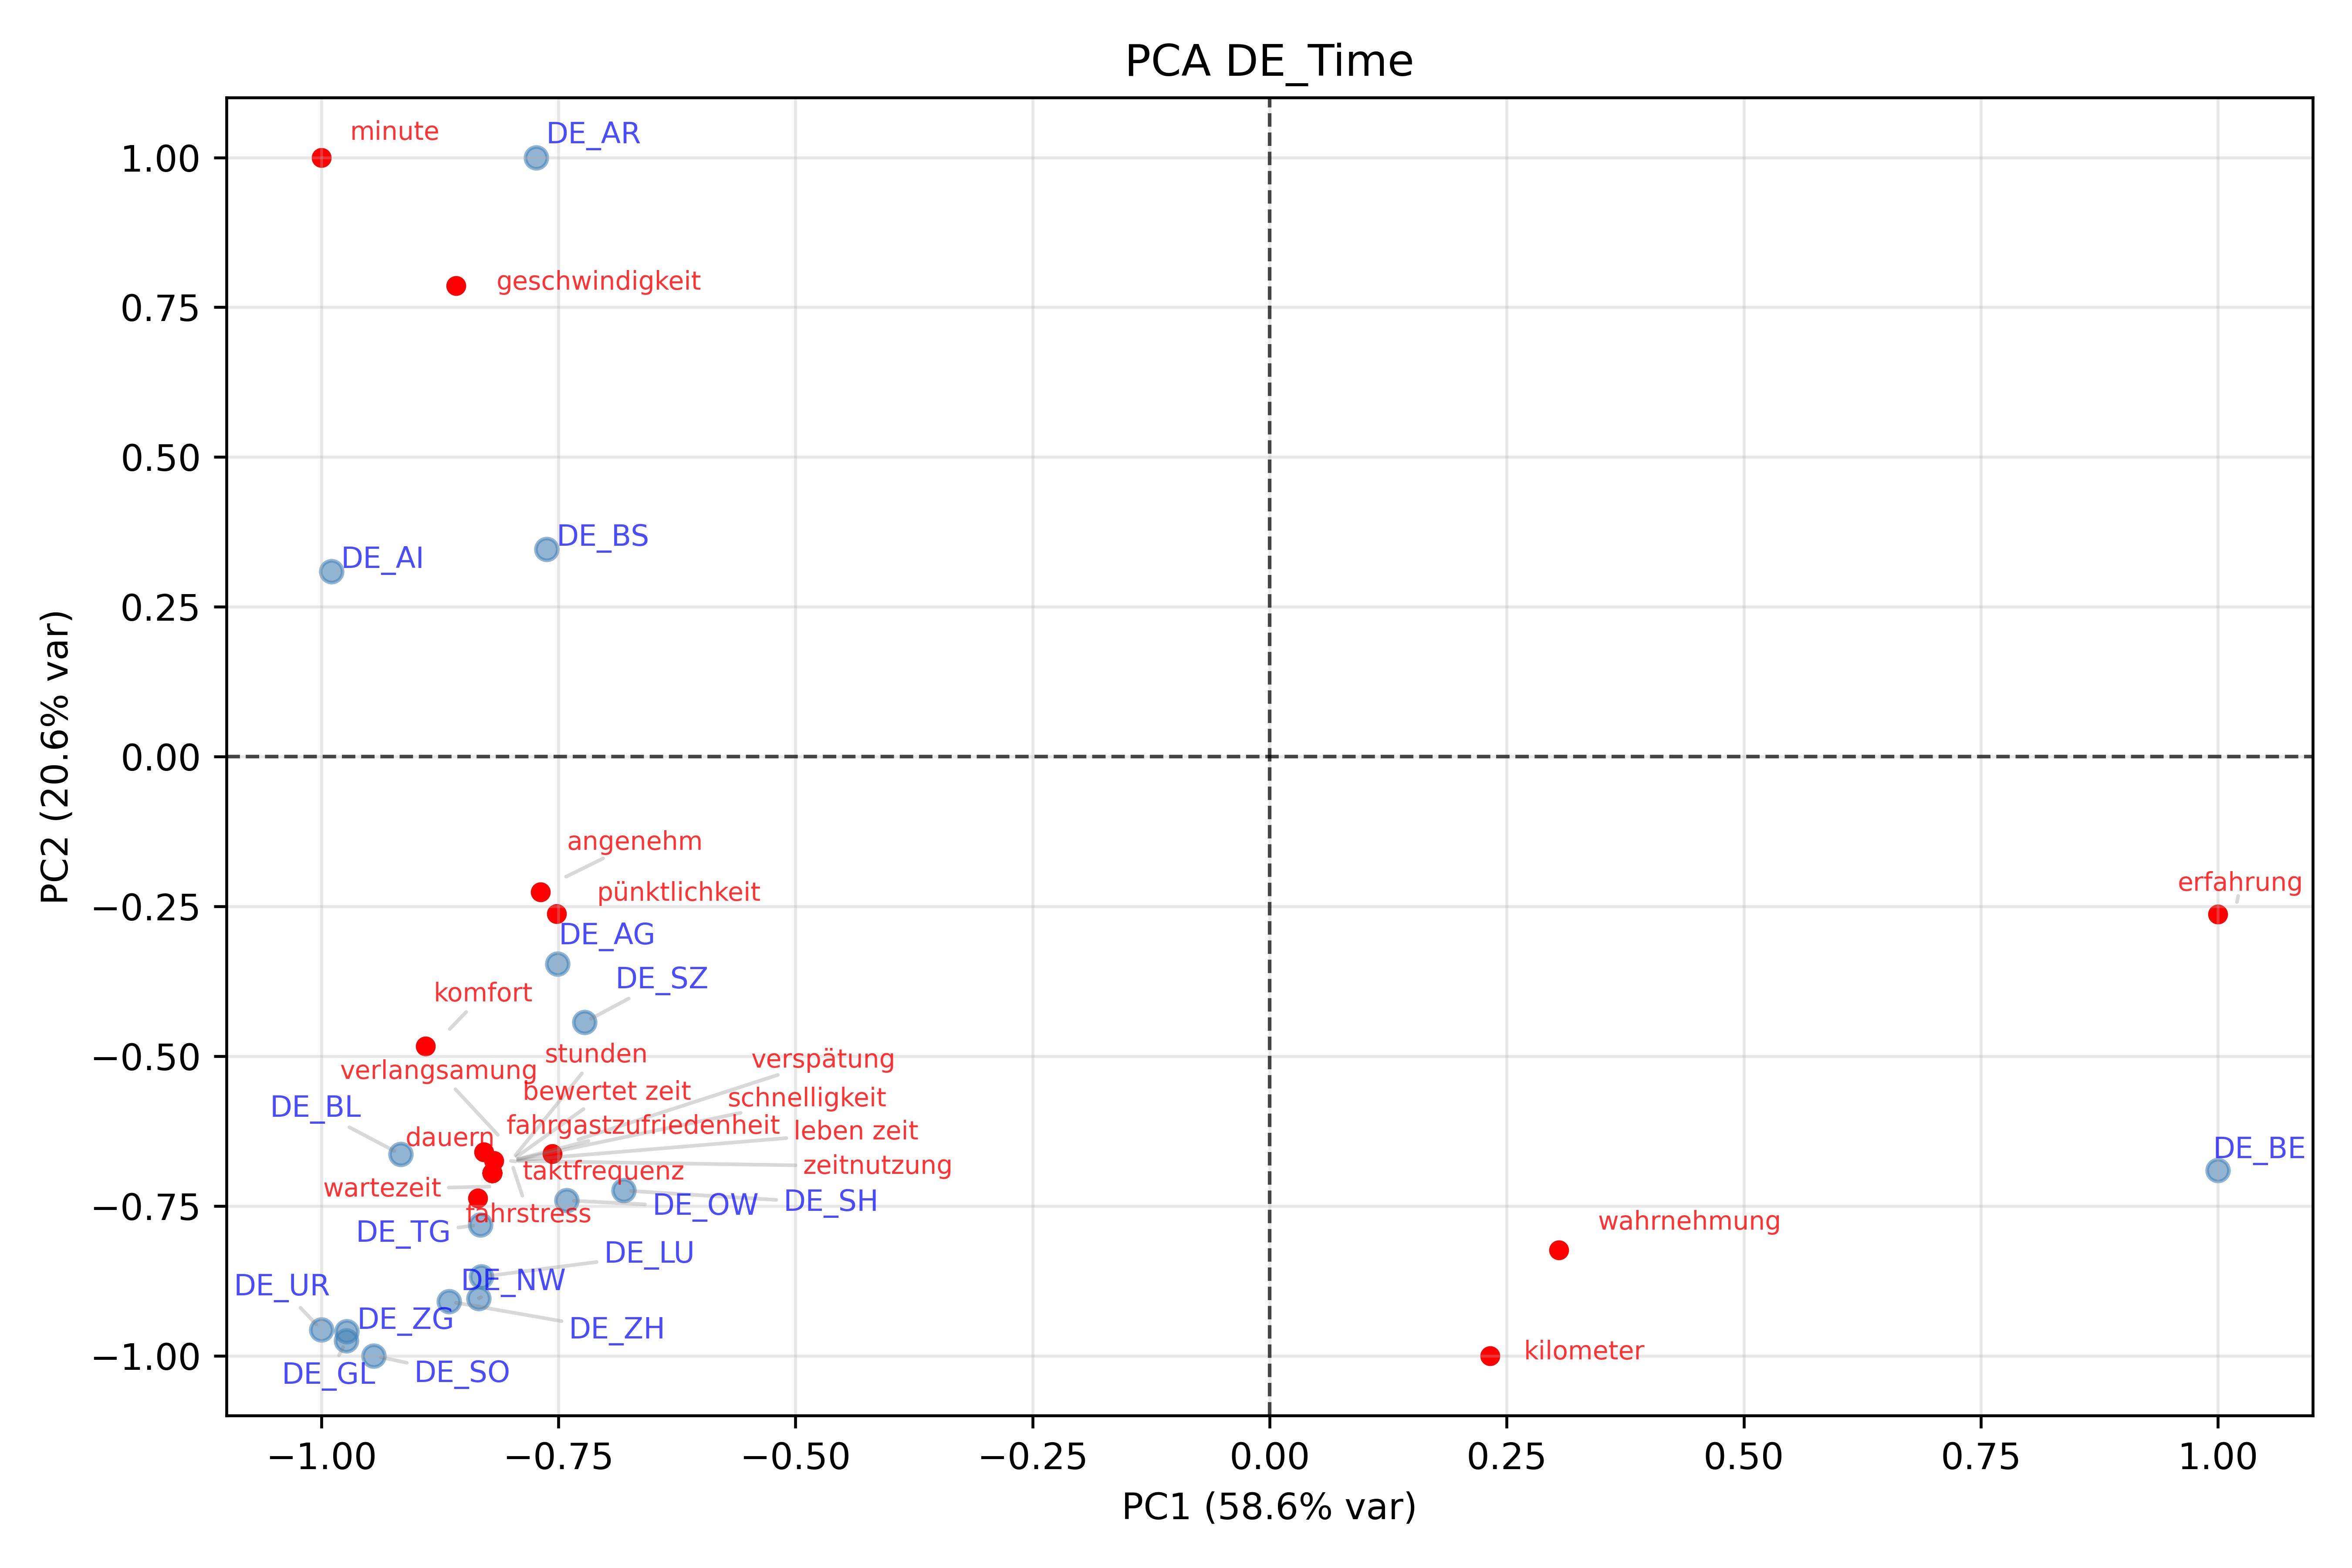
\includegraphics[width=0.95\linewidth]{Analysis/software/result/PCA_DE_Time.png}
    \caption{The German PCA confirms the strong prevalence of measurable time markers, with 
experiential notions appearing peripheral and weakly structuring the corpus.}
    \label{fig:PCA_DE_time}
\end{figure}

\newpage

\subsection{Analysis of PCA Results related to mobility}

Figure~\ref{fig:PCA_FR_mobility} shows a clear opposition between highly operational 
mobility notions and more capability-oriented terms. The first principal component captures the strong weight of "infrastructure", which dominates the positive side of the axis and forms the main structuring force in the corpus along with "coût", "accessibilité", "réseau transport" and "qualité desserte". 
Experiential or capability-related notions like "motivation mobilité", "apprentissage 
mobilité" or "habitus mobilité" cluster on the left very tightly together, indicating that they co-vary as a group but contribute only weakly to structuring differences between documents. The 
cantonal documents form a dense cluster near the negative side of the horizontal axis, except for Vaud and Bern, which are isolated at the positive extreme, similarly to the time PCA. This position suggests that VD relies more heavily 
on infrastructure and technical vocabulary than other French-speaking cantons, which 
use capability-based terms even more rarely than the others.

As shown in Figure~\ref{fig:PCA_DE_mobility}, the German corpus displays a similar 
structure, with "infrastruktur" and "kosten" anchoring opposite sides of the second 
principal component. Capability-related terms such as "mobilitätskompetenz", 
"bewegungsautonomie" or "mobilitätshabitus" cluster near the centre and form a dense 
semantic block. Their central position indicates that they vary little across the 
documents and are very underrepresented per table \ref{table:table_motility}; they are not the primary drivers of separation. The cantons again cluster 
tightly on the negative side of the horizontal axis, with BS, BL and BE positioned at the two extremes of the first two components. 
These outliers reflect a stronger emphasis on specific operational themes in these 
cantons, while the rest of the German-speaking corpus remains lexically homogeneous. 
Overall, measurable and infrastructural notions structure the corpus far more strongly 
than capability-related vocabulary.


\begin{figure}[H]
    \centering
    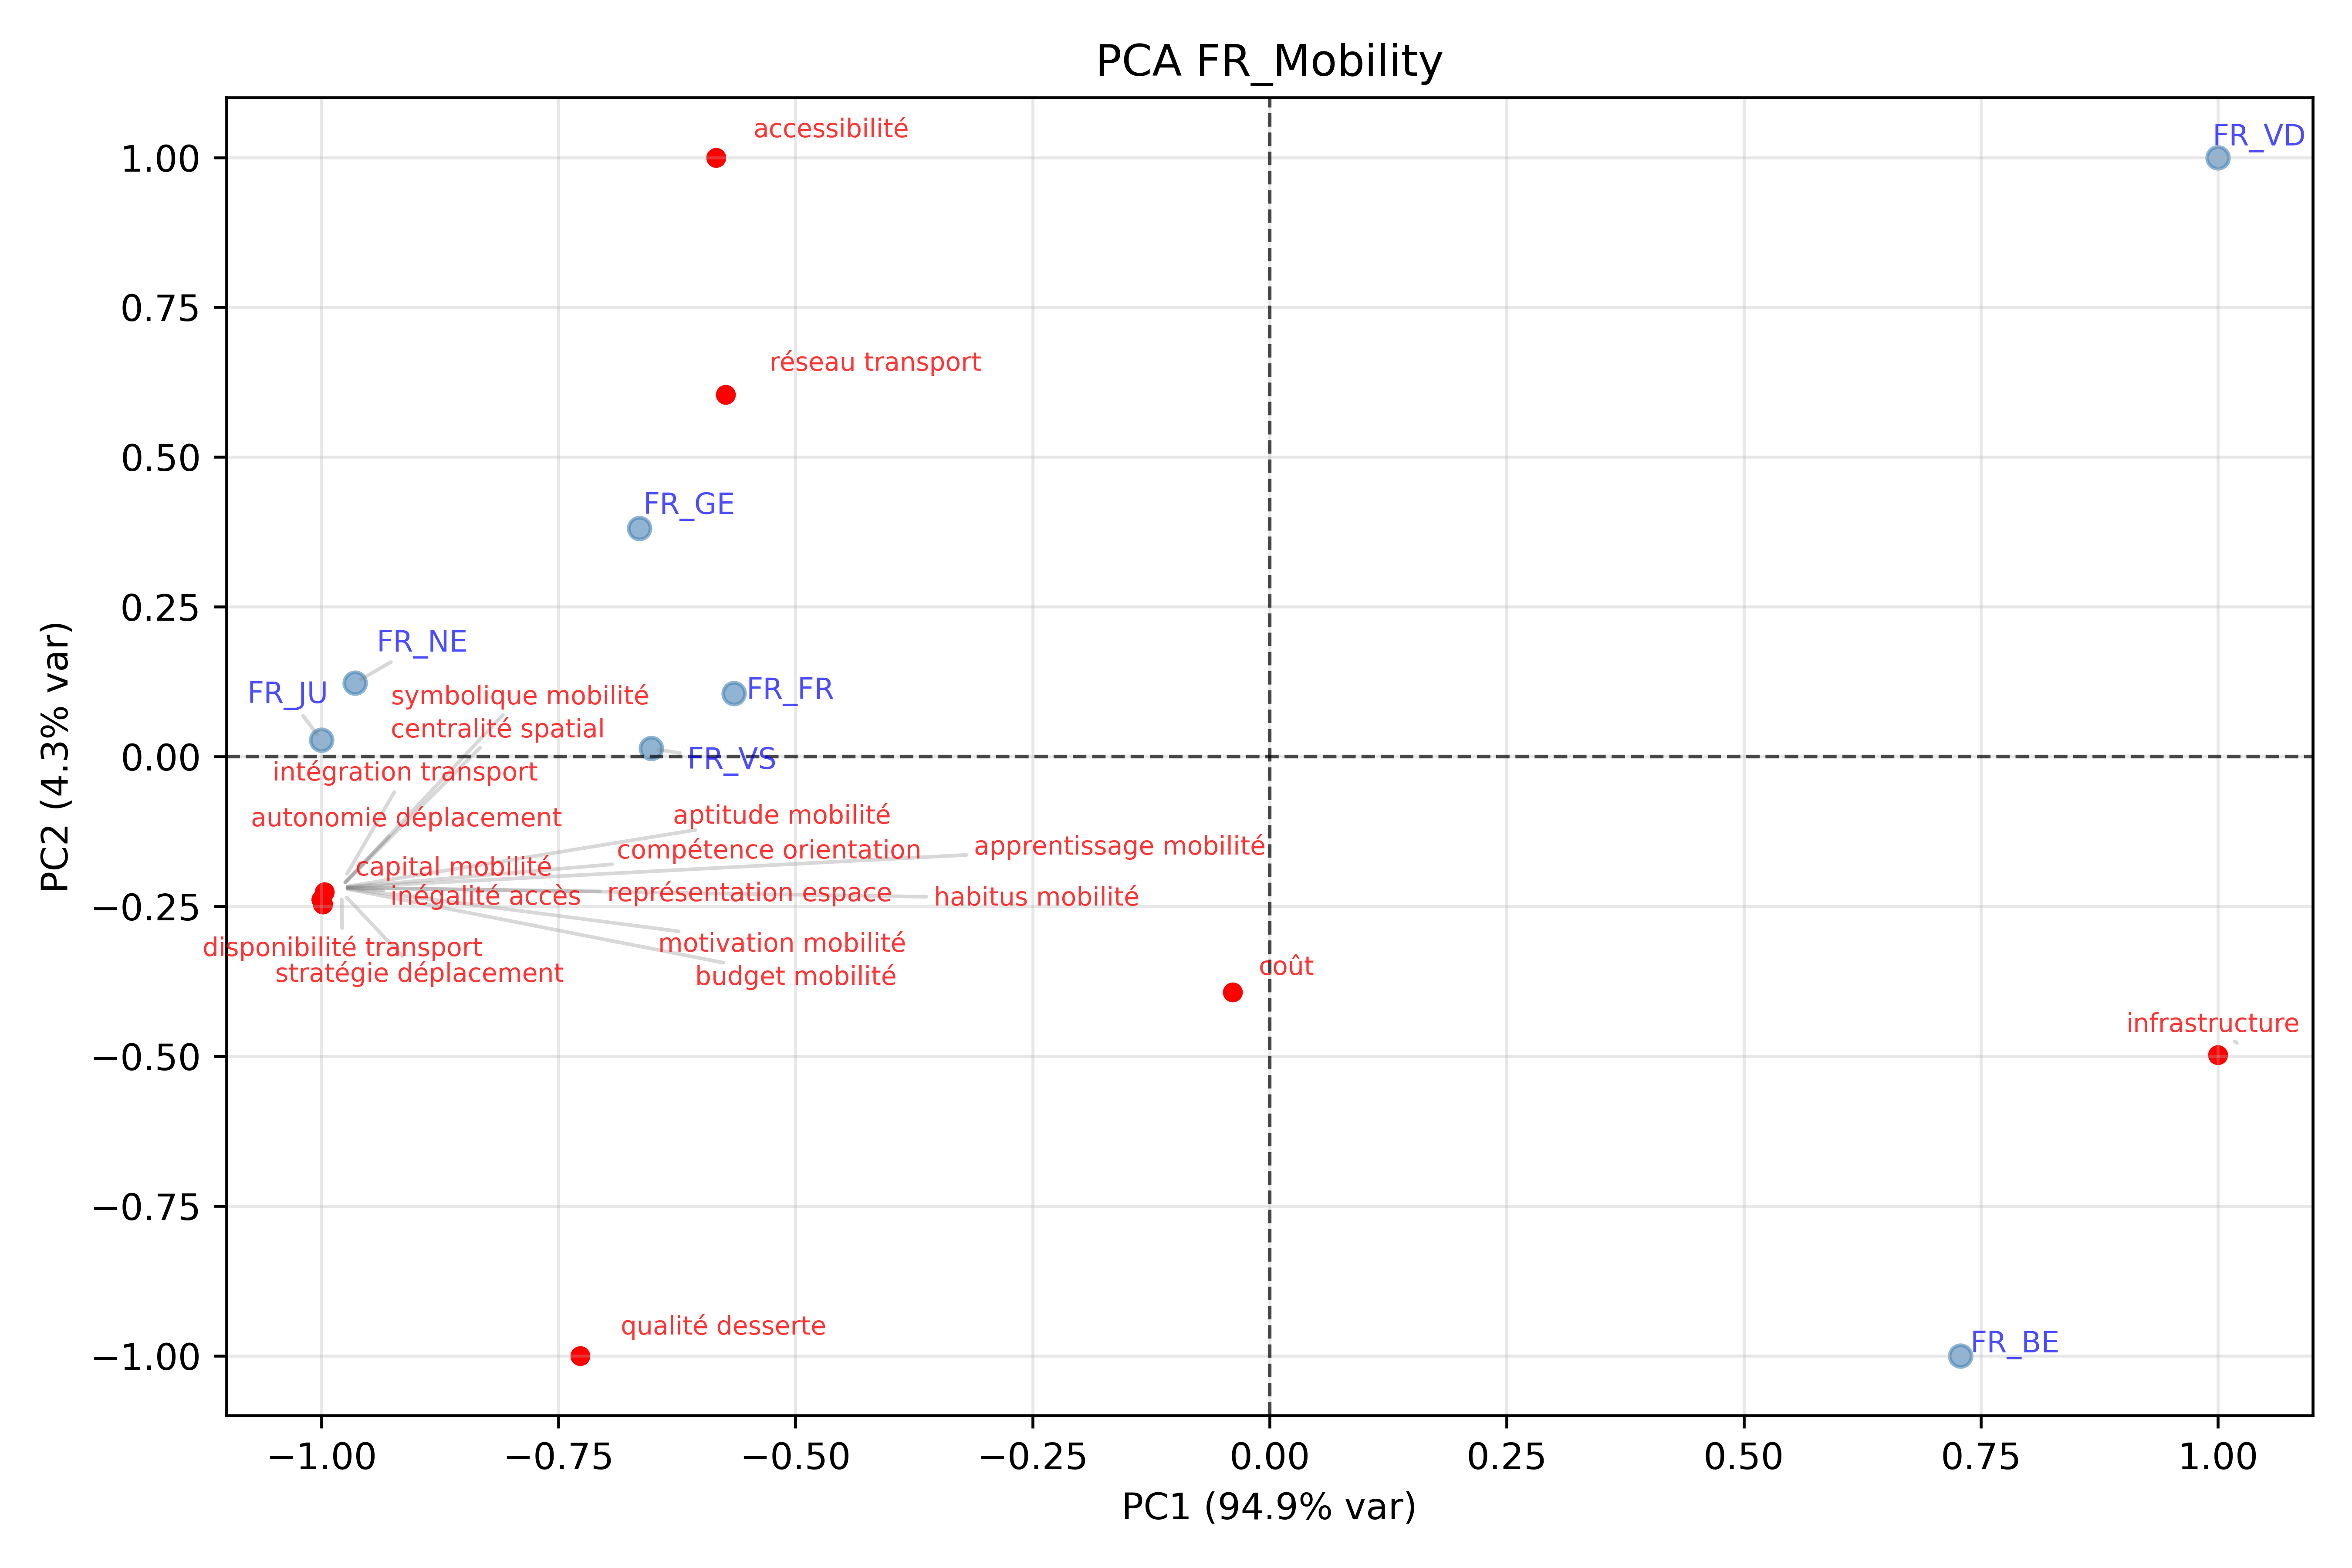
\includegraphics[width=0.95\linewidth]{Analysis/software/result/PCA_FR_Mobility.png}
    \caption{The French PCA reveals a strong axis contrasting infrastructure-focused terms with 
capability-oriented mobility notions, with VD standing apart from the other cantons.}
    \label{fig:PCA_FR_mobility}
\end{figure}

\begin{figure}[H]
    \centering
    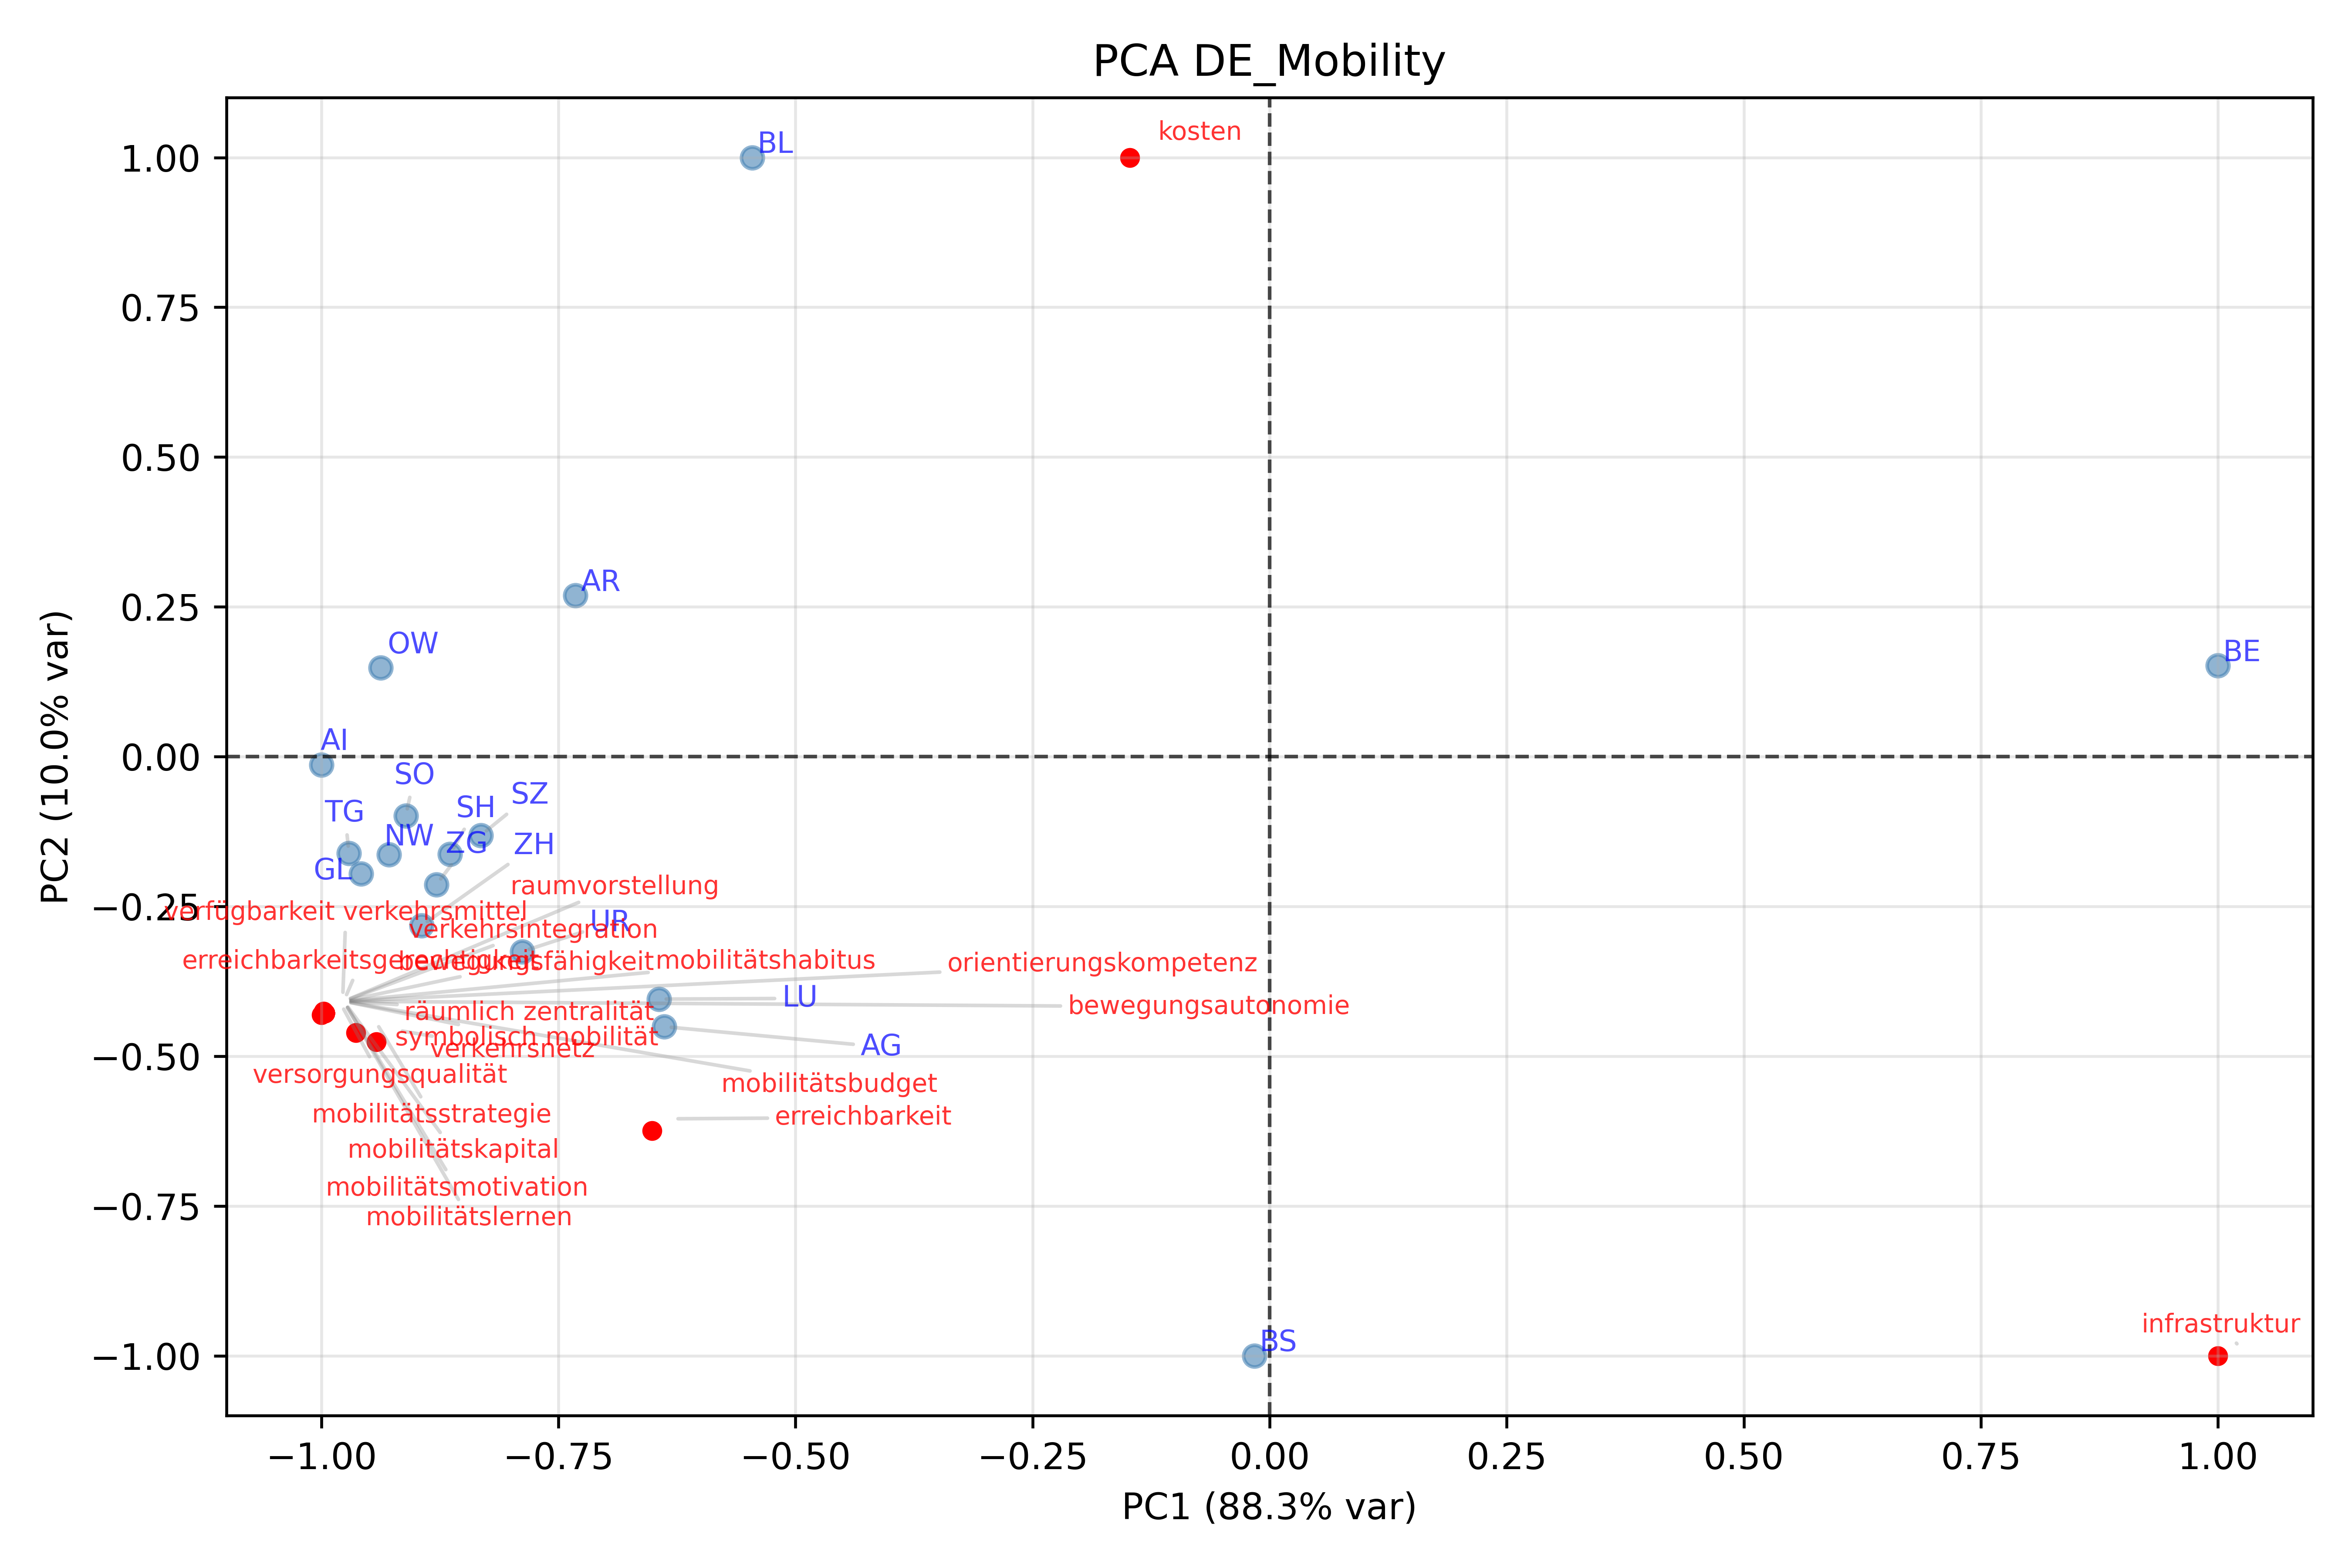
\includegraphics[width=0.95\linewidth]{Analysis/software/result/PCA_DE_Mobility.png}
    \caption{The German PCA highlights the dominance of operational and infrastructural mobility 
terms, while capability-related notions remain central and weakly discriminant.}
    \label{fig:PCA_DE_mobility}
\end{figure}

\subsection{Synthesis}

Combining the AFC results with the word occurrence analysis reveals a coherent narrative: Swiss spatial planning discourse is heavily skewed toward measurable, supply-oriented dimensions of mobility. Accessibility and physical time terms dominate both corpora, while motility and subjective time concepts are almost absent. This is consistent across French and German texts. 

Motility is conceptually underrepresented, indicating that planners primarily consider mobility as a function of infrastructure, services, and network performance rather than individual capabilities, skills or motivation. Time is similarly treated as a quantifiable variable, with minimal attention to comfort, perception or human experience. 

The combined word frequency and AFC results reinforce the conclusion that Swiss planning documents operationalize mobility and time in terms of provision and efficiency. Human-centered aspects, including cognitive, motivational and experiential dimensions, remain peripheral, reflecting a narrow and infrastructure-focused view of mobility.
